\documentclass{beamer}

\usepackage[utf8]{inputenc}
\usepackage{hyperref}

\usetheme{Berkeley}
\beamertemplatenavigationsymbolsempty
\setbeamertemplate{headline}{}
 
\title{Erfassen von Daten in FoodChain-Lab 1}
\date{}
 
\begin{document}
\maketitle

\section{ }

\subsection{Aufgaben}
\begin{frame}
	\begin{itemize}
		\item In diesem Tutorial werden wir zeigen, wie man mit unseren Excel-Templates Lieferdaten in FoodChain-Lab importiert.
		\item Wir werden zunächst die initialen Daten der Ausbruchsorte importieren und dann sukzessive Daten von Caterern und anderen Lieferanten mit Hilfe von autogenerieten Rückwärts- und Vorwärts-Tracing-Templates hinzufügen.
		\item In FoodChain-Lab ist es auch möglich das gesamte Liefernetz aus einer Excel-Datei zu importieren, aber dieses Feature wird hier nicht beschrieben. Das zugrundeliegende "All In One Template" kann heruntergeladen werden von: \url{https://github.com/SiLeBAT/BfROpenLabResources/raw/master/GitHubPages/templates/All_In_One_Template.xlsx}.
	\end{itemize}
\end{frame}
 
\subsection{1}
\begin{frame}
	\begin{center}
  		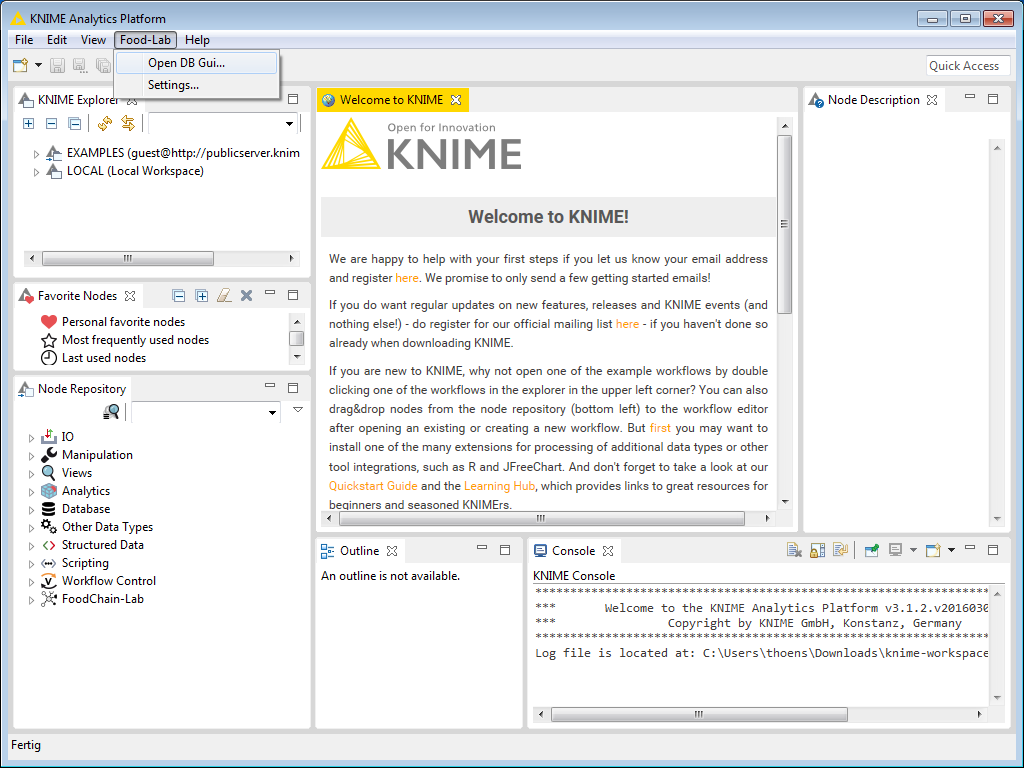
\includegraphics[height=0.6\textheight]{1.png}
	\end{center}
	\begin{itemize}
		\item Wählen Sie \textbf{Food-Lab $>$ Open DB Gui...} in der Menüleiste um die Datenbank-Oberfläche zu öffnen.
	\end{itemize}
\end{frame}

\subsection{2}
\begin{frame}
	\begin{center}
  		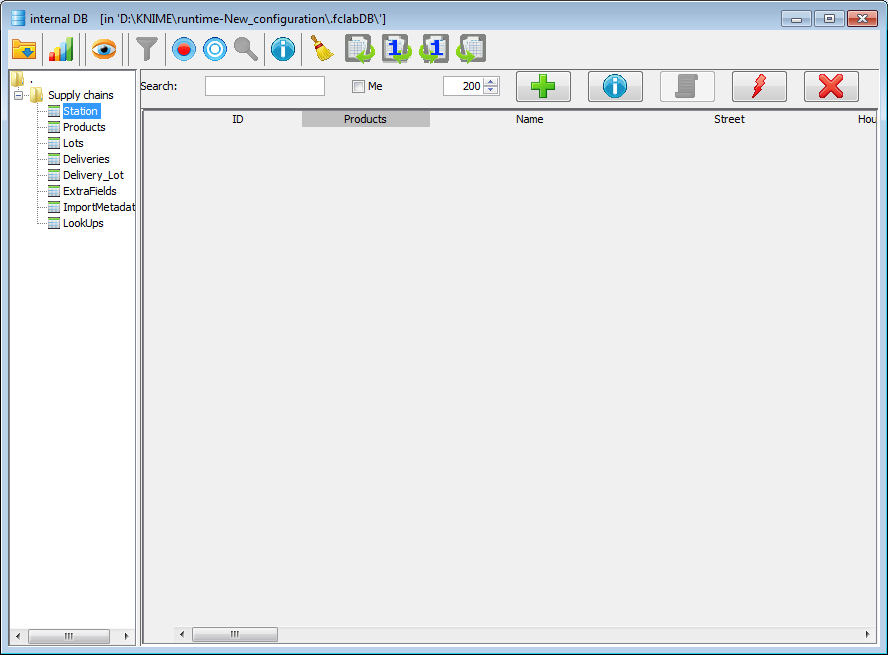
\includegraphics[height=0.45\textheight]{2.png}
	\end{center}
	\begin{itemize}
		\item Die Datenbank-Oberfläche erscheint nun.
		\item Hier können Sie Lieferdaten importieren, editieren und validieren.
		\item Um den Import zu starten, müssen Sie das "Start Tracing Template" herunterladen, ausfüllen und importieren.
		\item Das Template kann heruntergeladen werden unter: \url{https://github.com/SiLeBAT/BfROpenLabResources/raw/master/GitHubPages/templates/Start_Tracing_Template.xlsx}.
	\end{itemize}
\end{frame}

\subsection{3}
\begin{frame}
	\begin{center}
  		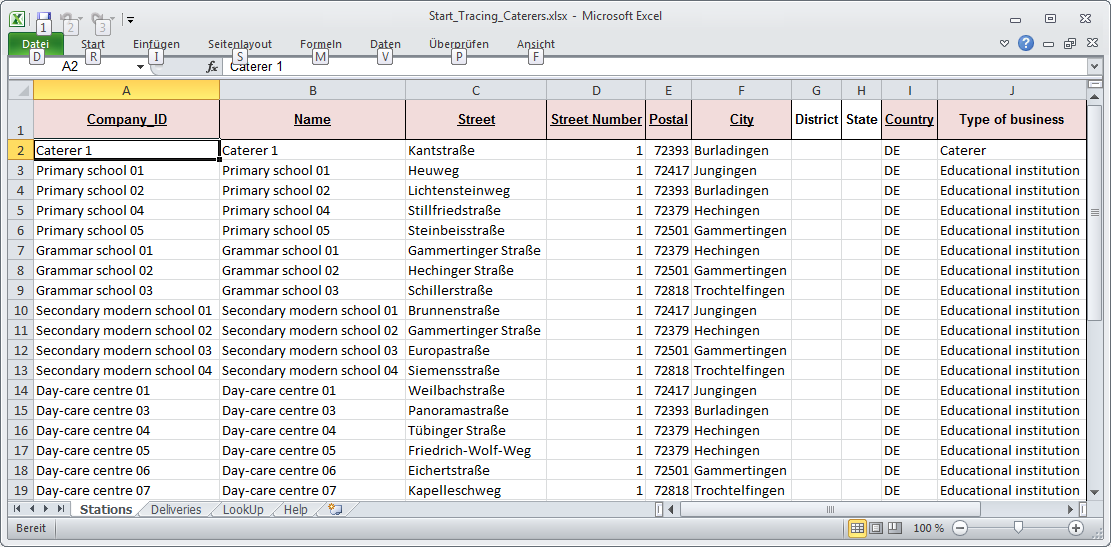
\includegraphics[width=0.95\textwidth]{3.png}
	\end{center}
	\begin{itemize}
		\item Für dieses Tutorial haben wir bereits ein ausgefülltes  "Start Tracing Template" vorbereitet.
		\item Downloaden sie es von \url{https://github.com/SiLeBAT/BfROpenLabResources/raw/master/GitHubPages/documents/Start_Tracing_Caterers.xlsx}.
		\item Im \textbf{Stations}-Blatt dieser Datei sind mehrere Bildungseinrichtungen (\textbf{Educational Institutions}) und zwei \textbf{Caterer} definiert.
	\end{itemize}
\end{frame}

\subsection{4}
\begin{frame}
	\begin{center}
  		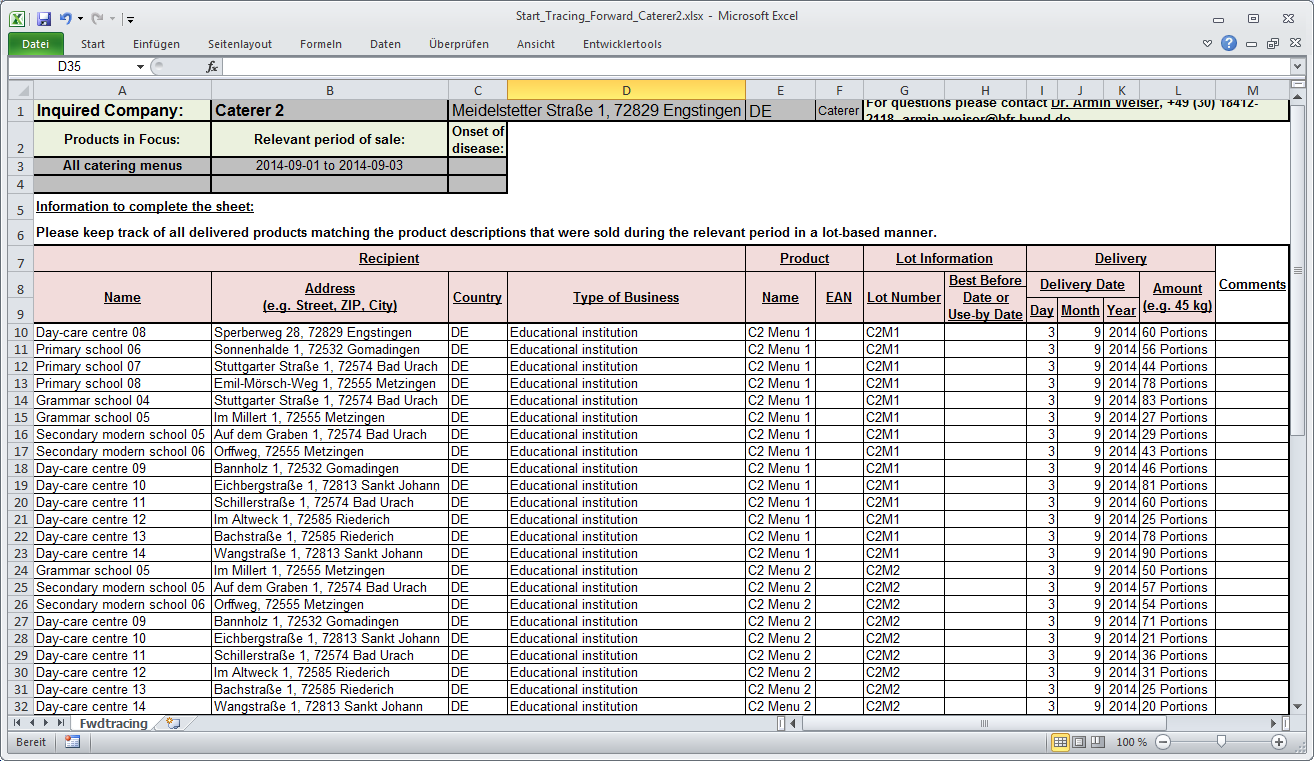
\includegraphics[width=0.95\textwidth]{4.png}
	\end{center}
	\begin{itemize}
		\item Krankheitsfälle wurden in diesen Bildungseinrichtungen, welche von \textbf{Caterern} beliefert wurden, gemeldet.
		\item Die Lieferungen von den \textbf{Caterern} an die Bildungseinrichtungen sind im \textbf{Deliveries}-Blatt definiert.
	\end{itemize}
\end{frame}

\subsection{5}
\begin{frame}
	\begin{center}
  		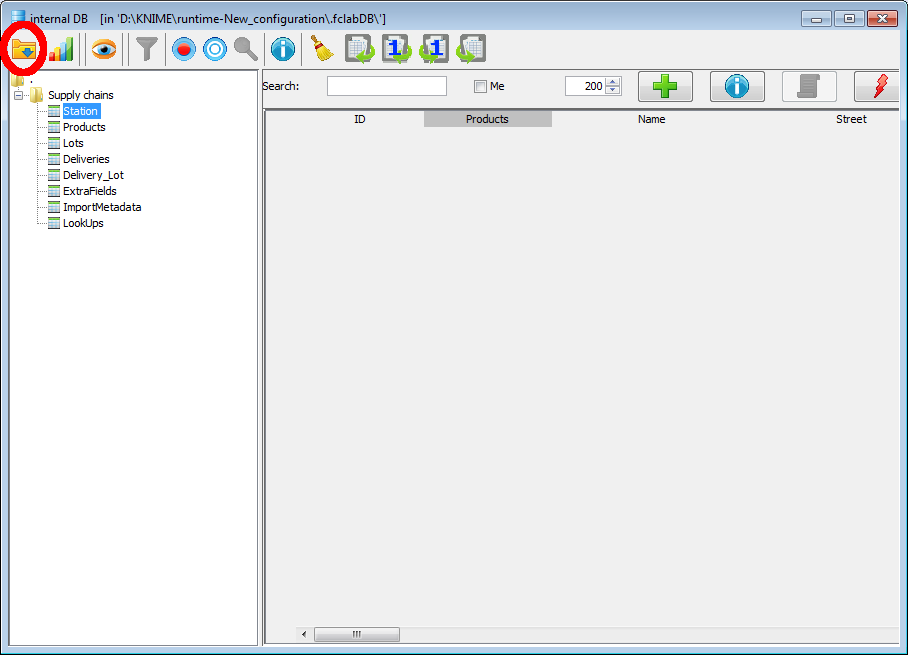
\includegraphics[height=0.6\textheight]{5.png}
	\end{center}
	\begin{itemize}
		\item Um diese Datei zu importieren klicken Sie auf  \textbf{Table import} in der linken oberen Ecke des Datenbankfensters.
	\end{itemize}
\end{frame}

\subsection{6}
\begin{frame}
	\begin{center}
  		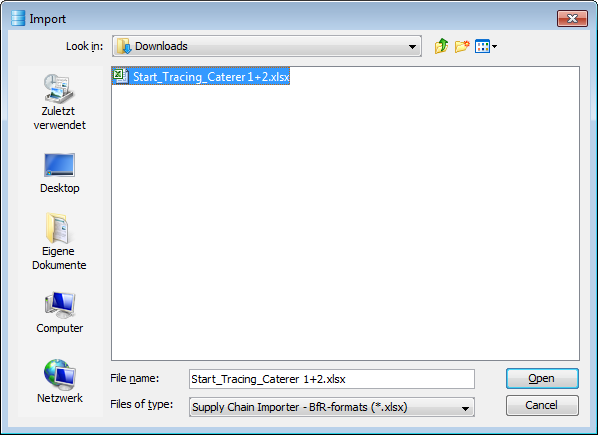
\includegraphics[height=0.5\textheight]{6.png}
	\end{center}
	\begin{itemize}
		\item In dem Dateidialog, der erscheint, selektieren sie "StartTracing\_Caterers.xlsx" und klicken Sie auf \textbf{Open}.
	\end{itemize}
\end{frame}

\subsection{7}
\begin{frame}
	\begin{center}
  		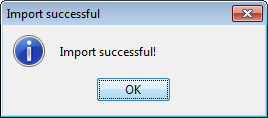
\includegraphics[width=0.4\textwidth]{7.png}
	\end{center}
	\begin{itemize}
		\item Sie werden darüber benachrichtigt, dass der Import erfolgreich war.
		\item Klicken Sie auf \textbf{OK}.
	\end{itemize}
\end{frame}

\subsection{8}
\begin{frame}
	\begin{center}
  		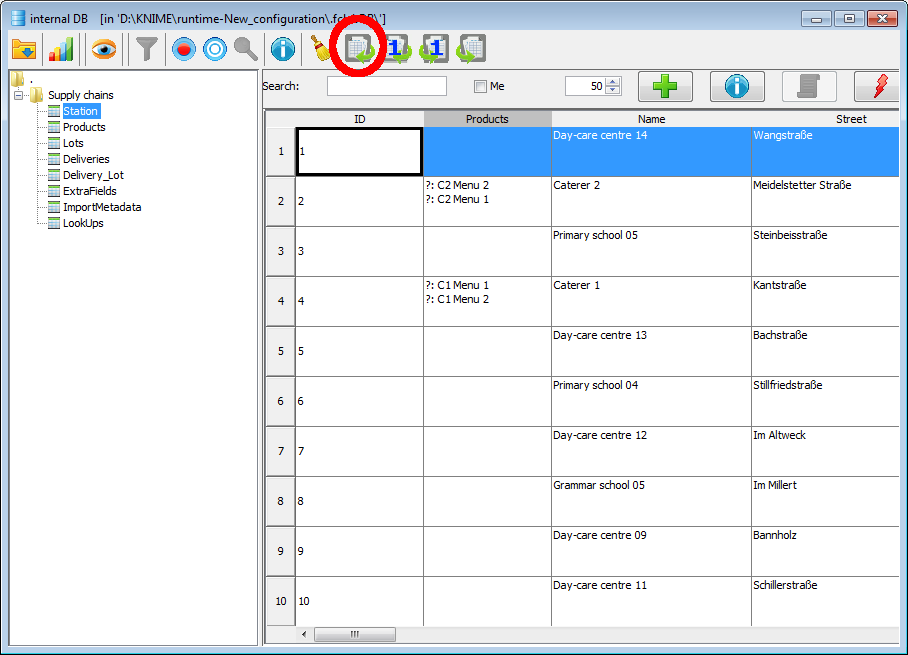
\includegraphics[height=0.5\textheight]{8.png}
	\end{center}
	\begin{itemize}
		\item Sie werden bemerken, dass im Datenbankfenster nun Einträge in der zuvor leeren Tabelle zu sehen sind.
		\item Nun wollen wir ein Rückwärts-Tracing von den Caterern aus durchführen, um zu sehen wo diese die Zutaten für die verschiedenen erworben haben.
		\item Drücken sie den Button zum Erzeugen von Rückwärts-Tracing-Templates (siehe roter Kreis).
	\end{itemize}
\end{frame}

\subsection{9}
\begin{frame}
	\begin{center}
  		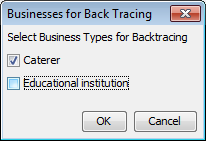
\includegraphics[width=0.4\textwidth]{9.png}
	\end{center}
	\begin{itemize}
		\item Da wir ein Rückwärts-Tracing für die Caterer durchführen wollen, wählen Sie nur \textbf{Caterer} und klicken sie auf \textbf{OK}.
	\end{itemize}
\end{frame}

\subsection{10}
\begin{frame}
	\begin{center}
  		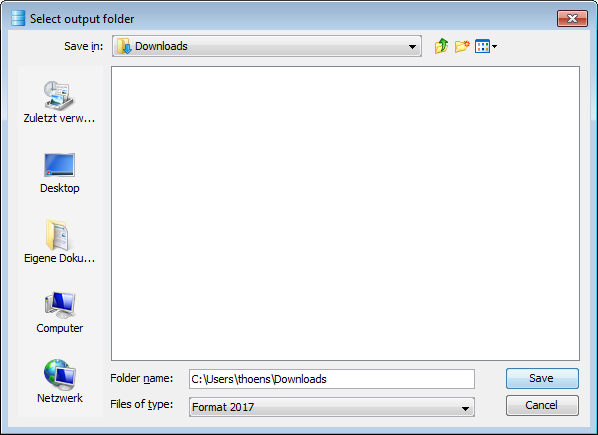
\includegraphics[height=0.5\textheight]{10.png}
	\end{center}
	\begin{itemize}
		\item In dem Dateidialog, der erscheint, können Sie den Ordner auswählen, in dem die generierten Templates gespeichert werden sollen.
		\item Wählen oder erzeugen Sie den gewünschten Ordner und klicken Sie auf \textbf{Save}.
	\end{itemize}
\end{frame}

\subsection{11}
\begin{frame}
	\begin{center}
  		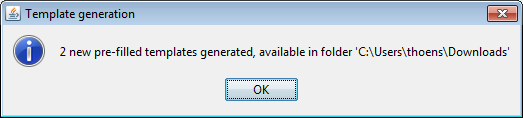
\includegraphics[width=0.8\textwidth]{11.png}
	\end{center}
	\begin{itemize}
		\item Sie werden benachrichtigt, dass zwei Templates generiert wurden.
		\item Klicken Sie auf \textbf{OK}.
	\end{itemize}
\end{frame}

\subsection{12}
\begin{frame}
	\begin{center}
  		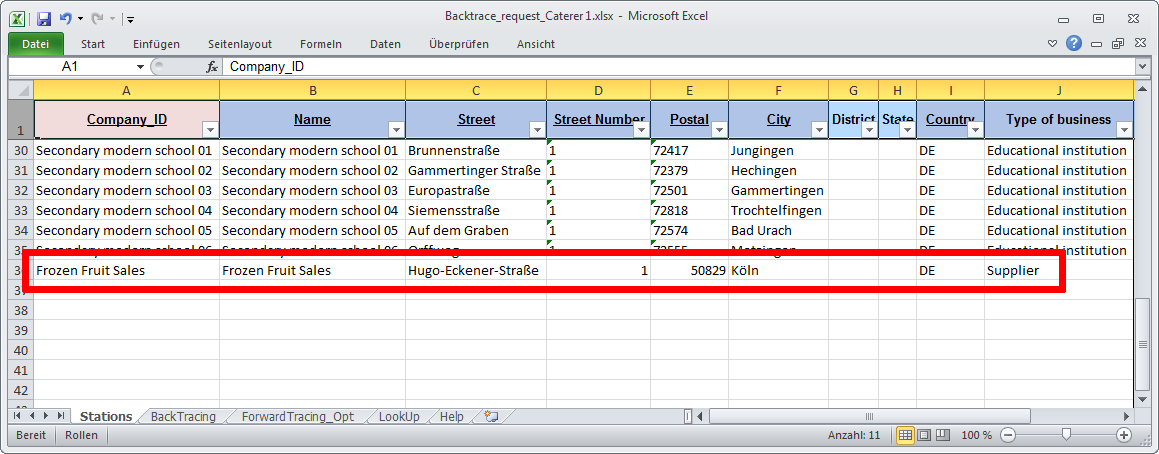
\includegraphics[width=0.95\textwidth]{12.png}
	\end{center}
	\begin{itemize}
		\item Um dieses Tutorial kurz zu halten, werden wir nur die Lieferungen von einem Lieferanten eingeben, "Frozen Fruit Sales".
		\item Geben Sie alle Informationen über "Frozen Fruit Sales" im \textbf{Stations}-Blatt der Datei "Backtrace\_request\_Caterer 1.xlsx" ein, wie im Screenshot zu sehen ist.
	\end{itemize}
\end{frame}

\subsection{13}
\begin{frame}
	\begin{center}
  		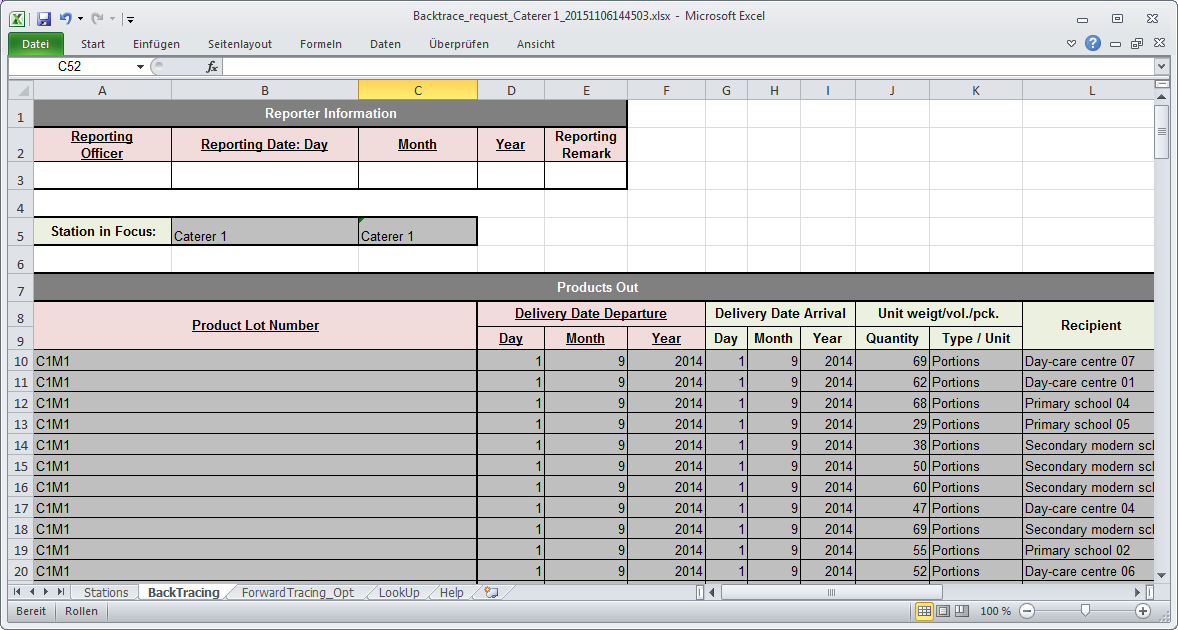
\includegraphics[width=0.95\textwidth]{13.png}
	\end{center}
	\begin{itemize}
		\item Wechseln Sie zum \textbf{BackTracing}-Blatt.
		\item Im \textbf{Products Out}-Bereich sind alle Lieferungen zu "Caterer 1" gelistet.
		\item Dies sind die Lieferungen, die wir aus "StartTracing\_Caterers.xlsx" importiert haben.
		\item Die Lieferungen gehören zu zwei Lots, "C1M1" und "C1M2".
	\end{itemize}
\end{frame}

\subsection{14}
\begin{frame}
	\begin{center}
  		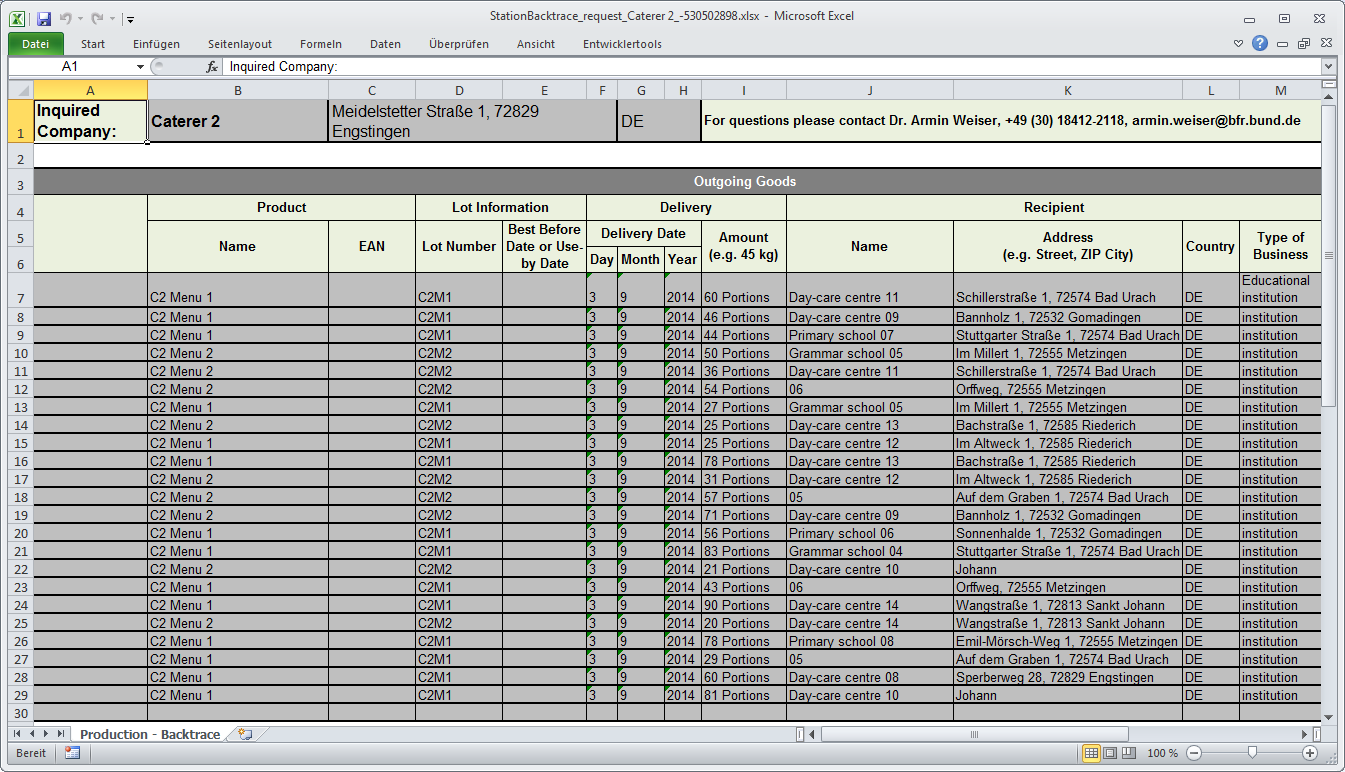
\includegraphics[width=0.74\textwidth]{14.png}
	\end{center}
	\begin{itemize}
		\item Scrollen Sie in den \textbf{Ingredients for Lot(s)}-Bereich.
		\item Hier können Sie alle Lieferungen eintragen, die "Caterer 1" empfangen hat und spezifizieren in welchen Lot die jeweilige Lieferung als Zutat gegangen ist.
		\item Geben Sie alle Informationen der "Frozen Strawberries"-Lieferung von "Frozen Fruit Sales" ein (siehe Screenshot).
		\item Speichern Sie das Dokument ("Backtrace\_request\_Caterer 1.xlsx").
	\end{itemize}
\end{frame}

\subsection{15}
\begin{frame}
	\begin{center}
  		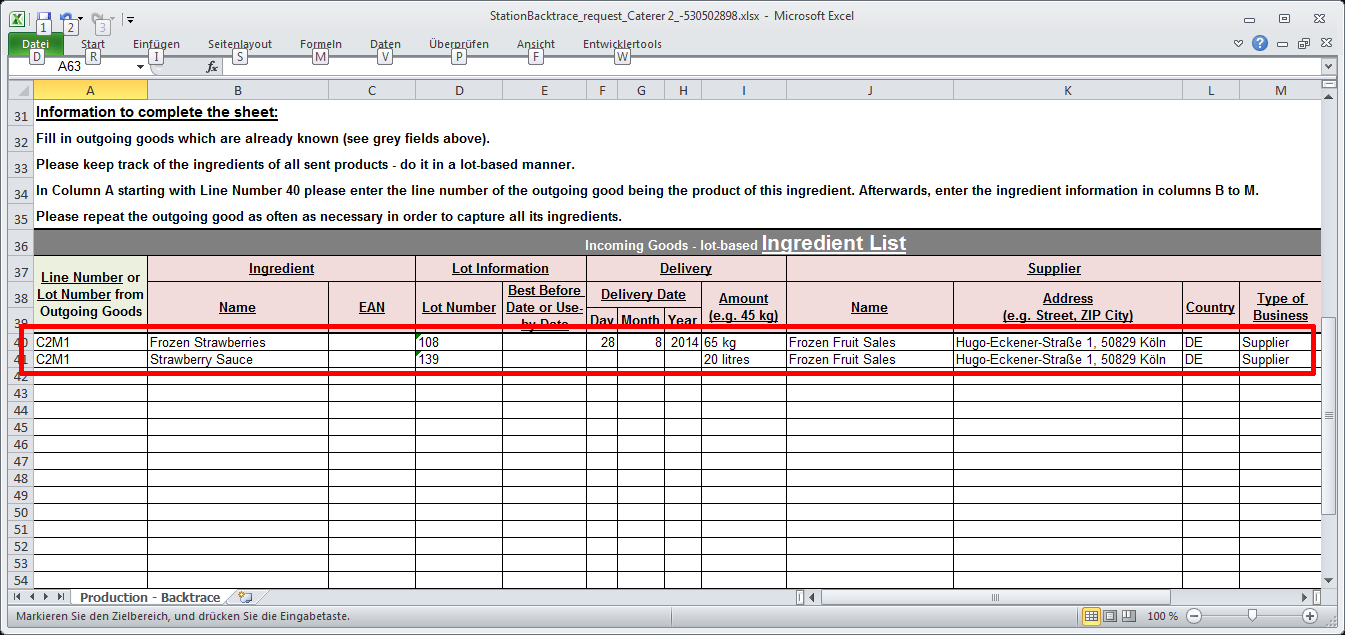
\includegraphics[width=0.95\textwidth]{15.png}
	\end{center}
	\begin{itemize}
		\item Nun öffnen Sie das andere generierte Template: "Backtrace\_request\_Caterer 2.xlsx".
		\item Fügen Sie "Frozen Fruit Sales" zu dem \textbf{Stations}-Blatt hinzu, so wie Sie es beim ersten Template gemacht haben.
	\end{itemize}
\end{frame}

\subsection{16}
\begin{frame}
	\begin{center}
  		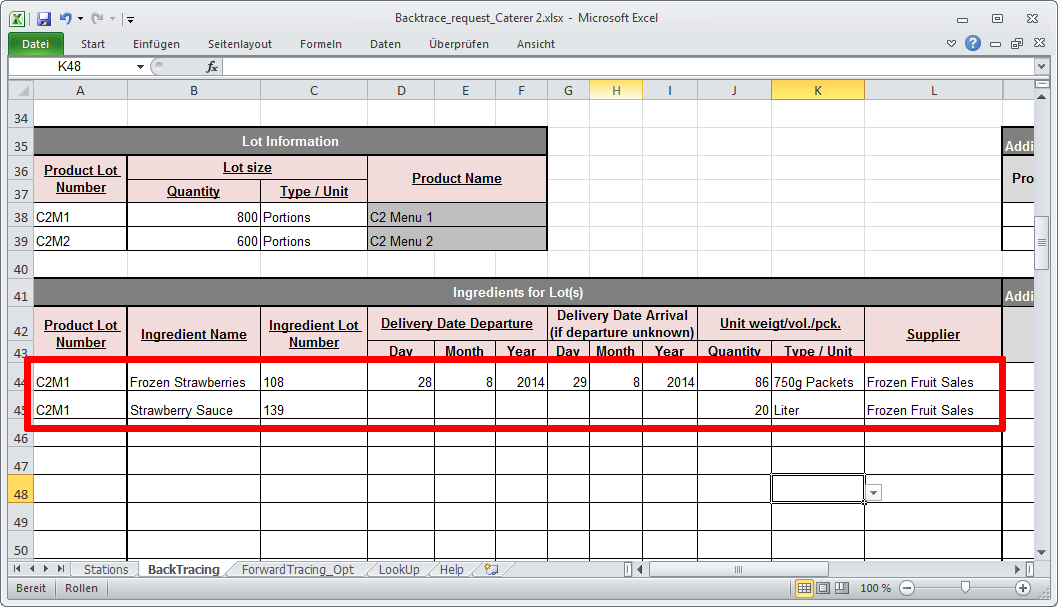
\includegraphics[width=0.95\textwidth]{16.png}
	\end{center}
	\begin{itemize}
		\item Wechseln Sie zum \textbf{BackTracing}-Blatt.
		\item Geben Sie die zwei Lieferungen vom Screenshot im \textbf{Ingredients for Lot(s)}-Bereich ein.
		\item Speichern Sie das Dokument ("Backtrace\_request\_Caterer 2.xlsx").
	\end{itemize}
\end{frame}

\subsection{17}
\begin{frame}
	\begin{center}
  		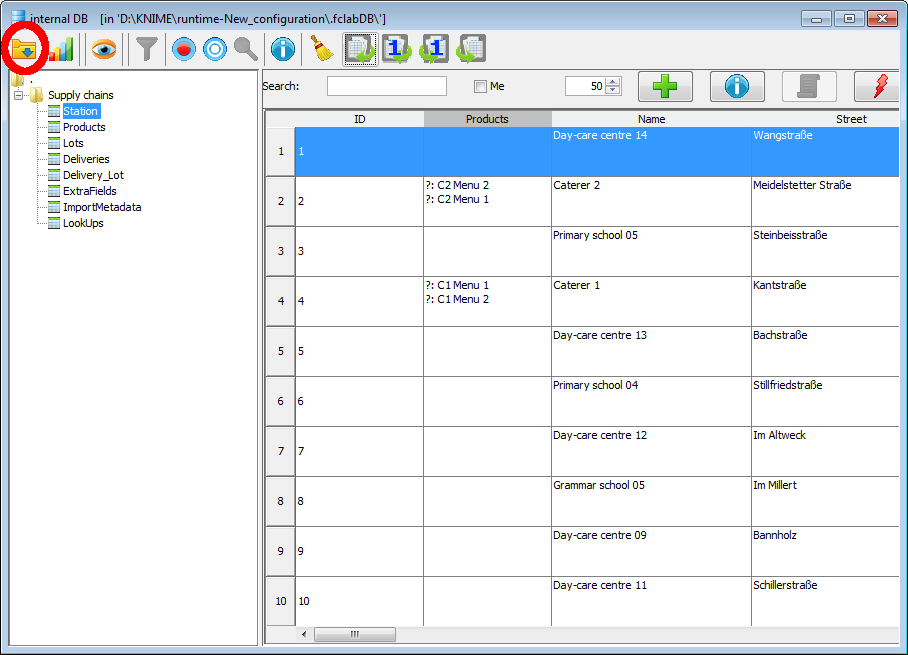
\includegraphics[height=0.6\textheight]{17.png}
	\end{center}
	\begin{itemize}
		\item Um die beiden Templates in die Datenbank zu importieren, klicken Sie den Button \textbf{Table import} in der linken oberen Ecke des Datenbank-Fensters.
	\end{itemize}
\end{frame}

\subsection{18}
\begin{frame}
	\begin{center}
  		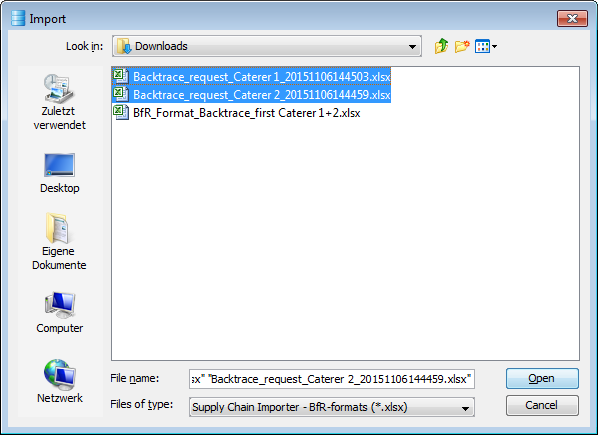
\includegraphics[height=0.5\textheight]{18.png}
	\end{center}
	\begin{itemize}
		\item Im Dateidialog, der erscheint, markieren Sie "Backtrace\_request\_Caterer 1.xlsx" und "Backtrace\_request\_Caterer 2.xlsx".
		\item Dann klicken Sie auf \textbf{Open}.
	\end{itemize}
\end{frame}

\subsection{19}
\begin{frame}
	\begin{center}
  		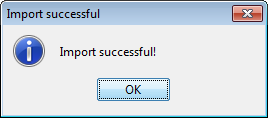
\includegraphics[width=0.4\textwidth]{19.png}
	\end{center}
	\begin{itemize}
		\item Sie bekommen eine Nachricht, dass der Import erfolgreich war.
		\item Klicken Sie auf \textbf{OK}.
	\end{itemize}
\end{frame}

\end{document}